\chapter{Estado de los recursos}
\label{chap:estadoInfraestructuraSistema}

\lettrine{C}{on} el fin de contextualizar los recursos que se utilizarán en este trabajo, en este capítulo se expone la situación actual de toda la infraestructura en lo relacionado al software que está en funcionamiento, a los recursos físicos de los que se compone, y al estado actual de las herramientas que rodean a dichos recursos.

\begin{section}{Infraestructura}
La infraestructura física donde se planea desplegar el servicio de virtualización, se encuentra localizada en el edificio del CITIC de la UDC, dentro de un rack alojado en su Centro de Proceso de Datos (CPD) \cite{citicUDC}. 
\begin{subsection}{Cómputo}
    La forman 5 nodos \textit{Lenovo NeXtScale nx360 M5} cada uno con dos procesadores Intel Xeon E5-2650, 128 GB de memoria RAM y una tarjeta gráfica Tesla M60,  y 3 nodos \textit{Dell EMC PowerEdge R740} cada uno con dos procesadores Xeon Gold 6146, 384 GB de memoria RAM y una tarjeta gráfica Tesla P40. Todos ellos aportan flexibilidad en cuanto a la escalabilidad de la infraestructura y ofrecen gran rendimiento de cómputo.
\end{subsection}
% Especificaciones principales de los nodos:
% \begin{itemize}
%     \item Lenovo NeXtScale nx360 M5: 
%         \begin{itemize}
%             \item CPU: Dos Intel Xeon E5-2650
%             \item Memoria: 128 GB
%             \item Tarjeta  gráfica: Tesla M60
%         \end{itemize}
%             Más información: \url{https://lenovopress.com/tips1195-nextscale-nx360-m5-e5-2600-v3}
%     \item Dell EMC PowerEdge R740:
%         \begin{itemize}
%             \item CPU: Dos Xeon Gold 6146
%             \item Memoria: 384 GB
%             \item Tarjeta gráfica: Tesla P40
%         \end{itemize}
%     Más información: \url{https://www.dell.com/es-es/work/shop/servidores-almacenamiento-y-redes/smart-value-poweredge-r740-server-standard/spd/poweredge-r740/per7400m}
% \end{itemize}
\begin{subsection}{Almacenamiento}
    El almacenamiento está colocado físicamente en la misma ubicación que los hosts pero en su abstracción lógica este es independiente y está separado de cada nodo. Está conformado por 13 discos duros SSD de 3.84 TB de capacidad, obteniendo así una cantidad total de casi 50 TB pero la capacidad útil es de 34 TB ya que se utiliza la configuración de almacenamiento RAID 5[Pal. \ref{itm:raid5}] para aporta mayor  integridad de los datos, mayor tolerancia a fallos y mayor ancho de banda. Los discos duros están colocados en una misma cabina donde forman un \textit{pool} de almacenamiento que se divide en cinco LUNs (\textit{Logical Storage Unit})[Pal. \ref{itm:lun}] de 2 TB cada una, representadas en el software de virtualización como cinco \textit{datastores} y que emplean el sistema de archivos VMFS propio de la compañía VMware y el cual optimiza el almacenamiento de máquinas virtuales.
    La configuración y gestión de este sistema se tiene que realizar al nivel de la capa física, por lo tanto si se quiere hacer un despliegue en el sistema de virtualización con una configuración de almacenamiento diferente a la existente, como por ejemplo un sistema RAID con diferentes características, sería necesario modificar la configuración del sistema físico pudiendo generar un gran coste de tiempo. Esto no permite ajustar de forma precisa y rápida las configuraciones que se necesitan para realizar despliegues sobre la infraestructura.
\end{subsection}

\begin{subsection}{Red}
    El sistema de almacenamiento forma una SAN, para ello las conexiones que se implementan entre los nodos y las cabinas donde se encuentran los discos duros son de tipo 10 Gbit. Para soportar esta conexión, cada cabina incorpora dos controladores SFP+[Pal. \ref{itm:sfp}]. Además, las cabinas de almacenamiento incorporan otros dos puertos de 1 Gbit para la administración de los discos. En esta estructura se utilizan los protocolos de red Ethernet y iSCSI. Finalmente, para mantener la disponibilidad del acceso al sistema de almacenamiento y las comunicaciones entre los nodos, cada uno de ellos se conecta a dos switches \textit{trunk} estableciendo rutas redundantes.
    Igual que con el sistema de almacenamiento, si se requieren realizar modificaciones sobre la red para adaptarse a los requisitos de un determinado despliegue habría que hacerlas directamente sobre la red física. Esto puede generar problemas en la conectividad del entorno a parte de generar gran coste de tiempo.
    % Todos los nodos están conectados a dos switches \textit{trunk} a través de los cuales se establecen conexiones redundantes para mantener la comunicación activa entre los nodos y el sistema de almacenamiento en caso de de que alguna falle. Estas conexiones son de tipo 10 GbitPara ello, las cabinas incorporan dos controladores con conexión SFP+[Pal. \ref{itm:sfp}] que se conectan a cada switch mediante dos puertos que aportan conectividad 10 Gb y, además, incorporan otros dos puertos con conectividad 1 Gb para la gestión de los discos. Estas conexiones utilizan los protocolos de red Ethernet y iSCSI, formando así, junto con el resto de componentes descritos, la estructura de una SAN [\ref{fig:esquemaentornoreal}].
\end{subsection}

% La gestión del almacenamiento se realiza en la capa física, el nivel más bajo por lo que la configuración de cada LUN que utilizan las máquinas virtuales desplegadas se tiene que hacer antes de conocer los requisitos necesarios de lo que se vaya a desplegar en la capa software. Esto provoca que si se quiere desplegar una máquina virtual con más capacidad de almacenamiento o con una estructura RAID diferente haya que crear una nueva LUN que se adapte a los requisitos.
% Esta gestión hace que el uso de recursos de almacenamiento no sea el óptimo ya que no permite ajustar de forma precisa y rápida cada configuración a los requisitos necesarios generando así mayor coste.

% \iffalse
% Los nodos acceden a los discos de almacenamiento a través de dos switches que al mismo tiempo dan conectividad entre los nodos formando una SAN. Los 10TB de capacidad están repartidos entre cinco DataStores, de 2TB cada uno. Una máquina virtual está alojada en un DataStore concreto pero puede tener ficheros alojados en varios almacenes de datos diferentes.
% Las conexiones entre dispositivos son Ethernet 10 Gigabit combinado con el protocolo de transporte ISCSI
% \fi
\end{section}

\begin{section}{Software}
\label{subsec:softwareinstalado}
Actualmente, el software desplegado sobre la infraestructura está formado por los productos de la compañía VMware, uno de los principales proveedores de software de virtualización, siendo \textbf{VMware vSphere}, versión 6.7, el principal componente ya que se utiliza para virtualizar parte de la infraestructura física y proporcionar las herramientas necesarias para gestionarla, sus principales componentes internos se describen a continuación.
\begin{figure}[h]
    \centering
    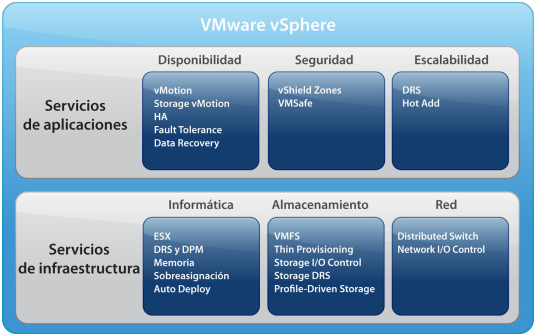
\includegraphics[width=0.75\textwidth]{imaxes/cap2recursos/contentVSphere}
    \caption{Componentes de VMware vSphere\cite{fotovSphere}}
    \label{fig:vSphere-components}
  \end{figure}
En cada nodo físico está instalado el \textbf{hipervisor ESXi}. Este es un hipervisor de tipo 1 o \textit{baremetal}, es decir, funciona directamente sobre el hardware sin necesidad de un sistema operativo adicional. Sobre los nodos corre el servicio \textbf{VMware vCenter Server} que actúa como centro de administración de todas las máquinas virtuales (VMs) y nodos que forman la infraestructura y, además, contiene una instancia embebida de \textbf{Platform Services Controller} (PSC) punto que centraliza el acceso a distintos servicios como APIs de VMware vCenter Server, servidor de licencias o el servicio de autenticación \textbf{vCenter Single Sign-On}, este último se utiliza para gestionar la autenticación de los usuarios registrados en VMware vCenter Server. El acceso e interfaz de VMware vCenter Server se realiza a través de la página \textbf{vSphere Web Client} donde el usuario puede autenticarse y gestionar las VMs y nodos que forman el entorno y el resto de servicios de VMware vSphere. Además, incorpora \textbf{vSphere Update Manager} que permite gestionar las actualizaciones de software de los componentes de VMware vSphere. Para administrar las conexiones de las VMs, vSphere utiliza \textbf{vSphere Distributed Switch} (vDS), un switch virtual que gestiona el tráfico de cada VM permitiendo indicar que interfaces físicas de cada nodo físico, configurar sus puertos, establecer políticas y crear subredes de forma centralizada. Finalmente, existen varios servicios de gran importancia que se encargan de mantener la disponibilidad de las VMs desplegadas sobre la infraestructura:

\begin{itemize}
    \item \textbf{vMotion} y \textbf{Storage vMotion}: el primero se encarga de migrar VMs de un nodo a otro de forma transparente y sin detener su ejecución, permitiendo planificar las migraciones. El segundo servicio se encarga de migrar los discos y configuración de una VM de un \textit{datastore} a otro sin interrumpir el servicio.
    
    \item \textbf{vSphere High Availability} (HA): En caso de que una VM deje de estar activa, este servicio intenta encenderla de forma automática en otro nodo del entorno. A diferencia de vMotion, este solo actúa en caso de que la VM o el nodo donde se encuentra la VM sufra un fallo y esta pase a estar no disponible. 
    
    %Proporciona escalabilidad gracias a su modelo Maestro - Esclavo, fiabilidad gracias a que no tiene dependencias con otros servicios y a que se puede comunicar con las máquinas a través de varios caminos, y usabilidad gracias a que tiene una interfaz sencilla.
    
    \item \textbf{vSphere Distributed Resource Scheduler} (DRS), \textbf{vSphere Distributed Power Management} (DPM) y \textbf{Sotrage DRS}: vSphere DRS genera recomendaciones sobre donde se debería desplegar una máquina virtual durante su creación, utiliza vMotion para migrar las VMs y así maximizar el rendimiento o para manterner la VM activa durante tareas de mantenimiento en un nodo. vSphere DPM se encarga de gestionar el consumo de energía de cada host según el rendimiento actual. Sotrage DRS se encarga de balancear la carga de almacenamiento y las operaciones de lectura y escritura entre los \textit{datastores} disponibles.
    % \item \textbf{Storage DRS}: balancea la carga de almacenamiento y las operaciones I/O entre los diferentes datastores disponibles.
    
    \item \textbf{vSphere Fault Tolerance}: gestiona una copia de todos los archivos y discos de cada VM sincronizada con los archivos originales. Este servicio usado con vSphere HA y vSphere DRS proporciona recuperación ante fallos automática y disponibilidad continua de las VMs, sin perdida de datos y sin pérdida de las conexiones establecidas. En caso de que una VM deje de estar disponible esta se reinicia en un nodo diferente. Este servicio está orientado a proteger aquellas tareas que requieren un alto rendimiento o que son críticas.
\end{itemize}
    % \item \textbf{vSphere Distributed Switch (vDS)}: habilita switches virtuales que se encargan de gestionar el tráfico de los hosts ESXi. Se utiliza para administrar la configuración de los puertos de cada host ESXi de forma centralizada, permitiendo crear redes y establecer políticas sobre el tráfico desde un único lugar. Desde aquí se establecen las conexiones de cada tipo de tráfico con las tarjetas de red físicas de cada host ESXi.
    % \item \textbf{ESXi}: Hipervisor propio de VMware, de tipo 1 o \textit{bare metal}[Pal. \ref{itm:baremetal}]. No requiere de sistema operativo para funcionar ya que funciona directamente sobre el hardware físico\cite{Esxi}. Este hipervisor está instalado en cada uno de los ocho nodos que forman la infraestructura.
    
    % \item \textbf{VMware vCenter Server}: servicio que actúa como un administrador central para todas las máquinas virtuales y hosts. Normalmente, los servicios descritos en este apartado están disponibles para una instancia de vCenter Server agrupados en un \textit{Platform Services Controller} (PSC) [Pal. \ref{itm:psc}]
    
    % \item \textbf{vCenter Single Sign-On}: es un servicio de autenticación. Permite que los usuarios solo se tengan que autenticar una vez cuando acceden al entorno de la infraestructura a través de vSphere Client, en lugar de tener que autenticarse varias veces en cada componente. Cuando el usuario se autentica por primera vez, este recibe un token que le permitirá autenticarse en el resto de componentes sin volver a introducir sus credenciales. También se encarga de la administración perfiles de usuarios y de los dominios de autenticación (esto permite usar directorios de usuarios externos).\label{itm:singlesingonEX}
    
    % \iffalse
    % \item \textbf{vSphere License Server}: permite gestionar e inventariar licencias para aquellos sistemas conectados a un \emph{Platform Services Controller}.
    
    % \item \textbf{VMware Certificate Authority}: provee con un certificado a cada nodo. está firmado por esta misma autoridad (VMCA).
    % \fi
    % \iffalse
    % \item \textbf{PostgreSQL}: distribución de la base de datos PostgreSQL para vSphere.
    % \fi
    % \item \textbf{vSphere Web Client} y \textbf{vSphere Client}: interfaz que permite conectarse a una instancia de vCenter Server para gestionar la infraestructura.
    
    
    % \iffalse
    % \item \textbf{vSphere ESXi Dump Collector}: permite configurar un host ESXi para que guarde su memoria en un servidor externo en lugar de en un disco cuando hay algún fallo crítico.
    % \item \textbf{vSphere Syslog Collector}: habilita logs de red. 
    % \fi
    % \item \textbf{vSphere Auto Deploy}: herramienta que permite desplegar gran cantidad de nodos físicos de forma automátizada.
    
    % \item \textbf{vSphere Update Manager}: permite gestionar de forma centralizada y automatizada las actualizaciones para hosts ESXi, para el hardware de las máquinas virtuales y para actualizar e instalar software de terceros en los hosts ESXi. Este componente se ejecuta desde VMware vCenter Server como un servicio y requiere conexión a la red externa para obtener las actualizaciones.
   
    % \item \textbf{vSphere Web Client}: interfaz web que permite acceder a vCenter Server de forma remota.
    
    % \item \textbf{vMotion}: permite la migración de máquinas virtuales de un host a otro de forma transparente y sin detener su ejecución. Permite planificar las migraciones de máquinas virtuales entre hosts que pueden pertenecer a distintos clusters.
    
    % \item \textbf{Storage vMotion}: permite migrar los discos y configuración de una máquina virtual de un \textit{datastore} a otro sin interrumpir el servicio.
    
    % \item \textbf{vSphere High Availability (HA)}: provee alta disponibilidad para las máquinas virtuales. En caso de que una máquina virtual deje de estar activa, este servicio intenta encender la máquina  virtual en otro host dentro del mismo cluster automáticamente. Este solo actúa en caso de fallo de un host, mientras que vMotion solo actúa cuando las migraciones se hacen entre hosts activos. Proporciona escalabilidad gracias a su modelo Maestro - Esclavo, fiabilidad gracias a que no tiene dependencias con otros servicios y a que se puede comunicar con las máquinas a través de varios caminos, y usabilidad gracias a que tiene una interfaz sencilla.
    
    % \item \textbf{vSphere Distributed Resource Scheduler (DRS)} y \textbf{vSphere Distributed Power Management (DPM)}: DRS genera recomendaciones sobre donde se debería desplegar una máquina virtual cuando se está creando, utiliza vMotion para mover las máquinas virtuales a través de los hosts de un cluster para maximizar el rendimiento o durante tareas de mantenimiento en un host. DPM se encarga de gestionar el consumo de energía de cada host según el rendimiento necesario.
    % \item \textbf{Storage DRS}: balancea la carga de almacenamiento y las operaciones I/O entre los diferentes datastores disponibles.
    
    % \item \textbf{vSphere Fault Tolerance}: crea una copia de todos los archivos y discos de cada máquina virtual sincronizados con los originales. Esto junto con vSphere HA y vSphere DRS, proporciona recuperación ante fallos y  disponibilidad continua de las máquinas virtuales de forma automática en caso de que la máquina virtual esté inactiva, sin perdida de datos y sin pérdida de conexiones de que había activas. Este servicio está orientado a proteger aquellas tareas que requieren un alto rendimiento o que son críticas.
    % \iffalse
    % habilitadas creando una copia de cada una  para usarla en caso de que la primera falle.
    % \fi
    % \item \textbf{vSphere Distributed Switch (vDS)}: habilita switches virtuales que se encargan de gestionar el tráfico de los hosts ESXi. Se utiliza para administrar la configuración de los puertos de cada host ESXi de forma centralizada, permitiendo crear redes y establecer políticas sobre el tráfico desde un único lugar. Desde aquí se establecen las conexiones de cada tipo de tráfico con las tarjetas de red físicas de cada host ESXi.
    
    % \item \textbf{Virtual Machine File System (VMFS)}: sistema de archivos de alto rendimiento nativo de VMware vSphere. Se utiliza para implementar los almacenes de datos de la infraestructura y está optimizado para el almacenamiento de máquinas virtuales.
\end{section}

\begin{figure}[hp]
    \centering
    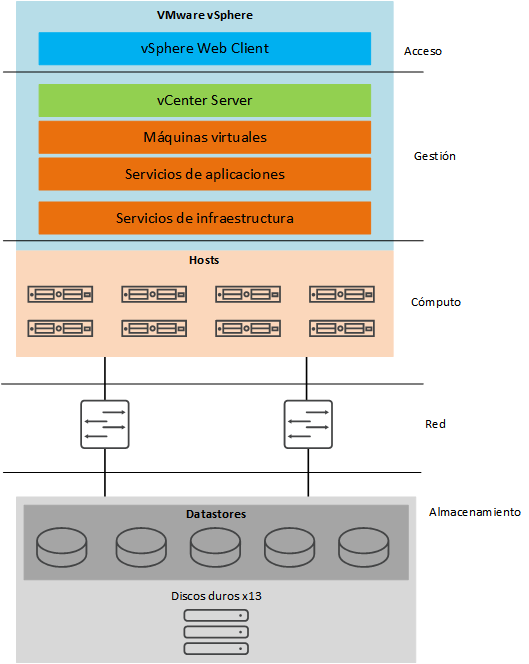
\includegraphics[width=0.6\textwidth]{imaxes/cap2recursos/recursosReal.png}
    \caption{Componentes físicos y software que forman la infraestructura actual.}
    \label{fig:infrastructure-components-production}
\end{figure}
\FloatBarrier

\begin{section}{Estado de la tecnología}
Con el desarrollo de las tecnologías web y la comercialización por parte de grandes empresas de su infraestructura los servicios \textit{Infrastructure as a Service} (IaaS) han ganado una popularidad considerable, con ello también se han desarrollado herramientas software dedicadas a la gestión infraestructura para la implementación de sistemas Cloud Computing. Algunas de estos servicios son VMware Cloud Foundation (creado en 2011), OpenStack (creado en 2010) o Apache CloudStack (creado en 2012). Estas herramientas construyen una infraestructura virtual sobre un conjunto de recursos físicos estandarizados que permite separar la administración de la capa física de la capa virtual, para simplificar y automatizar la gestión y escalabilidad de los recursos físicos y virtuales. Esto persigue reducir costes de gestión de la infraestructura y aumentar la disponibilidad del servicio, es decir, aumentar la eficiencia de la infraestructura física.
%   la disponibilidad del servicio, la red, y la seguridad del servicio, con lo que se consigue reducir el coste y el tiempo de gestión y configuración, mejorando la eficiencia de infraestructura física.
Si bien en el mercado existen varias alternativas que se pueden desplegar\footnote{OpenStack y Apache CloudStack entre otras.} sobre la infraestructura existente, finalmente, para cumplir los objetivos de este proyecto se ha escogido el producto \textbf{VMware Cloud Foundation} (VCF) ya que se integra perfectamente con los componentes de VMware ya instalados en la infraestructura y, por lo tanto, su mantenimiento a largo plazo es más sencillo. Desplegar un producto de una compañía diferente podría producir problemas de compatibilidad entre versiones a largo plazo, a pesar de que este se pueda integrar con el software VMware vSphere. Utilizando los productos de un mismo proveedor se asegura el soporte de las diferentes versiones del software instalado y la obtención del máximo rendimiento de cada componente.
Para poder usar este software es necesaria la adquisición de licencias, estas se organizan por componente y por número de hosts sobre los que se va a instalar el producto. Aunque tienen un coste elevado, este producto aporta grandes beneficios en cuanto a la gestión del SDDC.
% A la hora de alcanzar los objetivos descritos en este proyecto se nos plantea la duda de que solución software desplegar ya que actualmente existen tres principales alternativas en el mercado, VMware Cloud Foundation, OpenStack y Apache CloudStack. Cada una de ellas ofrece diferentes características con diferentes requisitos que se pueden adaptar mejor o peor al entorno de despliegue, pero después de comprobar esos aspectos tenemos claro que la \underline{solución elegida es VMware Cloud Foundation}.

\begin{subsection}{VMware Cloud Foundation}

    Esta solución de VMware virtualiza todas las capas de la infraestructura combinando cuatro de sus productos. Utiliza \textbf{VMware vSphere} para virtualizar y gestionar el cómputo, \textbf{VMware vSAN} para virtualizar y gestionar el almacenamiento, \textbf{VMware NSX-T} para la virtualización y gestión de la red, y \textbf{VMware vRealize} para gestionar las operaciones de la infraestructura virtual como el aprovisionamiento de recursos o la gestión de \textit{logs} centralizada. Todos juntos, estos servicios convierten el CPD en un \textit{Software Defined Datacenter} (SDDC), un entorno donde existe una infraestructura física que se abstrae en una capa virtual para separar la gestión de ambas y poder modificar la infraestructura virtual según las necesidades de los usuarios sin necesidad de modificar la configuración de la infraestructura física. Gracias a esa estructura obtiene las siguientes características:
\begin{itemize}
    \item \textbf{Servicios software con integración nativa}: ofrece un conjunto de servicios software para el almacenamiento, red, seguridad y gestión de la cloud. Estos servicios se integran de forma nativa con la infraestructura minimizando las tareas de configuración y administración.
    \item \textbf{Escalabilidad y elasticidad de los recursos}: la capacidad de la infraestructura se puede modificar de forma sencilla gracias a la automatización del ciclo de vida de todos los elementos y al desacople entre las dos capas (la física y la virtual).
    \item \textbf{Supervisión de los recursos}: ofrece supervisión de los recursos con reconocimiento de aplicaciones y solución de problemas, permitiendo conocer todos los eventos que tienen lugar en la infraestructura. También permite establecer políticas de seguridad en cuanto al acceso a los recursos y la red.
    \item \textbf{Aprovisionamiento automatizado}: permite la otención de recursos de forma automática incluyendo servicios de red, almacenamiento y cómputo. Los componentes de la infraestructura virtualizada se encargan de la reserva de los recursos y de todas las operaciones necesarias para llevarla acabo.
    %todos los componentes necesarios para formar un SDDC son desplegados automáticamente por VMware Cloud Foundation, incluyendo los recursos informáticos, los componentes de almacenamiento, los de red y los de administración.
    \item \textbf{Ciclo de vida automatizado}: automatiza las operaciones previas, iniciales y posterios de los recursos de la plataforma para simplificar y coordinar su gestión. En estas tareas se incluye desde el despliegue de la plataforma y su implementación, el aprovisionamiento de nuevos recursos físicos y la instalación de actualizaciones para cada componente software.
   
%    \iffalse 
%     \item \textbf{Experiencia de usuario simple}: gracias a la gran cantidad de procesos automatizados.
%     \item \textbf{Escalabilidad modular}: el sistema y la infraestructura se puede escalar de forma sencilla.
%     \item \textbf{Cloud híbrida}: da la posibilidad de conectar una Cloud pública con una Cloud privada y así tratar ambas como una única Cloud.
%     \fi
\end{itemize}
\begin{figure}[h!]
    \centering
    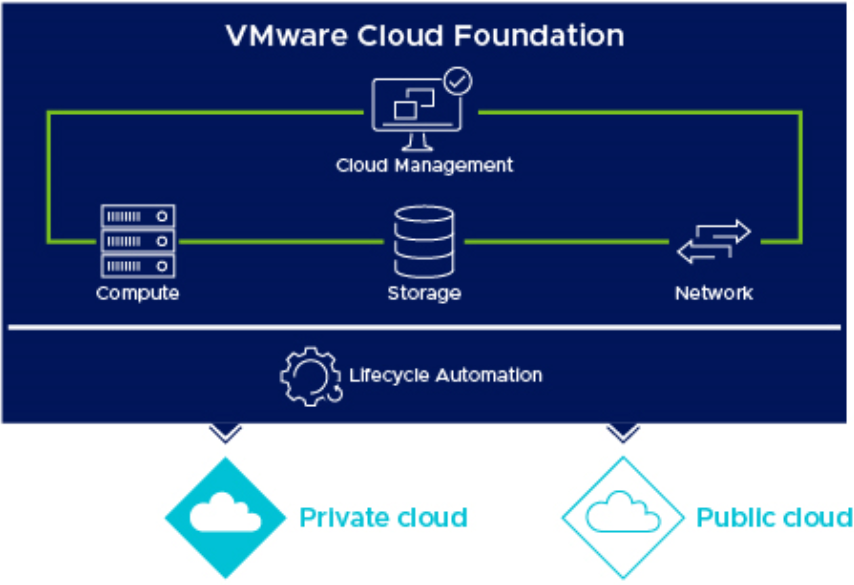
\includegraphics[width=0.6\textwidth]{imaxes/cap2recursos/overviewCF.png}
            \caption{Resumen partes de VMare Cloud Foundation.}
    \label{fig:Cloud-Foundation-Overview}
    \end{figure}
    \FloatBarrier
    \begin{figure}[h]
        \centering
        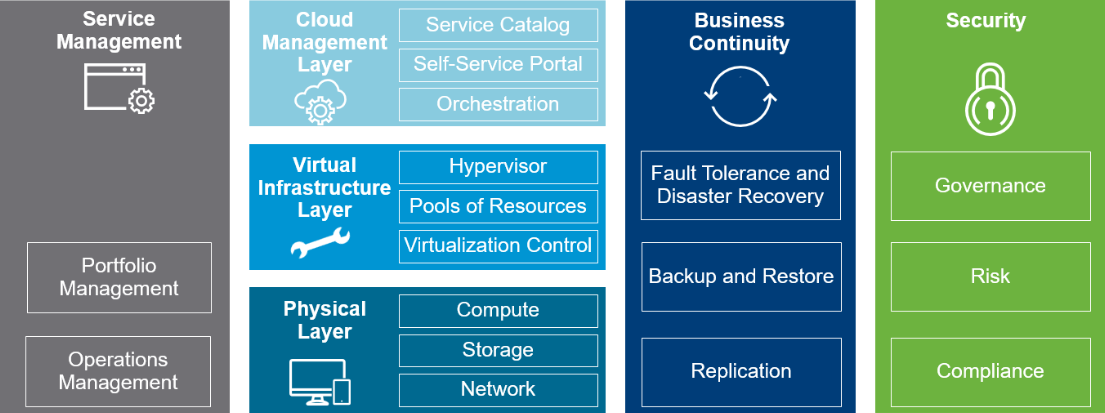
\includegraphics[width=0.8\textwidth]{imaxes/cap2recursos/SDDCoverview.png}
        \caption{Elementos de un SDDC gestionado con VMware Cloud Foundation.}
        \label{fig:layers-Sddc}
    \end{figure}
    \FloatBarrier
% VMware Cloud Foundation permite reducir el tiempo de mantenimiento ya que todo está controlado por el software que integra todos los componentes, automatizando gran parte de las operaciones y el ciclo de vida de todos los elementos desde su creación, como puede ser el control de versiones de cada elemento, los perfiles de usuario y las máquinas virtuales creadas, además de proporcionar una plataforma de acceso para que cada usuario pueda gestionar sus recursos. Además, su arquitectura se divide en entornos aislados administrados bajo demanda desde un entorno principal. Cada uno de esos entornos tiene un conjunto de recursos dedicados cuyas capacidades se pueden ajustar para proporcionar determinadas características, como por ejemplo alta disponibilidad, mayor capacidad de almacenamiento o mayor capacidad de cómputo. 

% \iffalse
% *****************************************************\\
% También permite separar las cargas de trabajo mediante Dominios según el tipo de trabajo que se va a realizar, pudiendo acceder a cada uno de ellos de forma separada.\\
% *****************************************************\\
% \fi

%  en cuanto integración nativa con los componentes ya instalados y a que su mantenimiento es más sencillo, se ha elegido este paquete ya que es más rentable que otras opciones. \\
% Si bien VMware ofrece plugins para conectar sus componentes con otras soluciones, como es el caso de OpenStack \cite{opestackintegrated}, estos no ofrecen el rendimiento que da la integración nativa, además, en caso de recibir actualizaciones, habría que actualizar cada componente de forma individual aumentando el riesgo de incompatibilidades con el resto de elementos del sistema, mientras que Cloud Foundation gestiona todo el ciclo de vida de cada actualización para cada componente, permitiendo comprobar si existe alguna incompatibilidad con el resto de versiones antes de aplicar una actualización. En definitiva, VmWare Cloud Foundation simplifica el proceso de instalación, configuración, gestión, y mantenimiento, tanto para los usuarios como para el administrador del sistema.
\end{subsection}

\begin{subsection}{Componentes de VMware Cloud Foundation \cite{componentesCloudFound}}
\label{subsubsect:cfcomponents}

% El SDDC de VMware Cloud Foundation está dividido en varias capas y módulos con las cuales se gestiona todas las partes de la infraestructura [Fig. \ref{fig:sddcoverview}]. Cada una de estas capas incluye una serie de productos y servicios, con unas funciones concretas que permiten gestionar un entorno complejo de una forma más sencilla. Las partes de esta infraestructura son las siguientes:
% \begin{itemize}
%     \item \textbf{Capa de Infraestructura física}: Es la base de la infraestructura y en ella residen los componentes físicos de almacenamiento, red y cómputo.
%     \item \textbf{Capa de Infraestructura Virtual}: Se encuentra sobre la capa física y se encarga de realizar las tareas de acceso a los recursos físicos para controlar su aprovisionamiento.
%     \item \textbf{Capa de Gestión Cloud}: Es la capa superior y se dedica a las tareas de consumo de los recursos, es decir, realiza peticiones a las capas inferiores para la obtención de los recursos.
%     \item \textbf{Capa de Gestión de Servicios}: Esta capa se centra en el mantenimiento de la arquitectura gestionando el ciclo de vida, la monitorización, logs y alertas de los componentes. 
%     \item \textbf{Capa de Gestión de Operaciones}: La función de esta capa es la monitorización de la capa de infraestructura física, de la capa de infraestructura virtual y de los flujos de trabajo de los usuarios.
%     \item \textbf{Capa de Continuidad del Servicio}: Contiene elementos que ayudan a que el servicio se mantenga activo y a evitar la pérdida de información crítica, proveyendo copias de seguridad, restauración y recuperación ante desastres.
%     \item \textbf{Capa de Seguridad}: Se encarga de que todos los componentes de la infraestructura estén bien delimitados para establecer un nivel de seguridad.
% \end{itemize}
Ya se ha visto que VCF está formado por cuatro productos principales de VMware. En este apartado se describirán las características de esos cuatro componentes más el servicio que los coordina\footnote{Las características del componente VMware vSphere son las mismas que las descritas en el punto \ref*{subsec:softwareinstalado}}. Se utilizará la versión 4.0 de VMware Cloud Foundation lo cual implica que se implementarán las versiones 4.0 de SDDC Manager, 7.0.0 de VMware vSphere, 7.0.0 de VMware vSAN, 3.0 de VMware NSX-T y 8.1 de VMware vRealize Suite.
% En VMware Cloud Foundation existen diversos productos y servicios, algunos son requeridos para construir la instancia mínima de un SDDC y otros ofrecen servicios adicionales que incrementan el rendimiento de la infraestructura. A continuación se describen aquellos componentes necesarios para la instalación mínima de VMware Cloud Foundation y que se usarán en la implementación de este proyecto:
\begin{subsubsection}{SDDC Manager}
    SDDC Manager se encarga de gestionar el ciclo de vida de todos los componentes de VCF, esto incluye el despliegue de cada uno, su configuración y la obtención e instalación de actualizaciones. Centraliza la gestión de las licencias y certificados de cada componente y administra el aprovisionamiento de nuevos recursos físicos para el SDDC y los ya existentes.
\end{subsubsection}
\begin{subsubsection}{VMware vSAN}
    VMware vSAN virtualiza el almacenamiento del SDDC. Permite gestionar de forma centralizada desde la interfaz de vSphere Web Client el sistema de almacenamiento sin necesidad de tener que modificar la configuración física, como es el caso de las LUNs de la infraestructura actual. Trata todos los recursos de almacenamiento como un único elmento denominado \textit{datastore} sobre el cual se pueden establecer políticas incluso a nivel de VM lo cual aporta gran flexibilidad. El acceso por parte de cada nodo al \textit{datastore} se realiza con el protocolo IP a través de una subred dedicada al servicio. Con VMware vSAN, el \textit{datastore} esta formado por discos de almacenamiento se organizan en grupos ligados a un nodo (un máximo de cinco grupos por nodo). Los grupos pueden tener configuración \textit{Hybrid} que combinia discos HDD y SDD, o configuración \textit{All-Flash} que solo utiliza SSD y por lo tanto tiene mayor rendimiento. Dentro de cada grupo existe un disco de caché y al menos un disco de capacidad donde se almacenan los datos persistentes\cite{operacionesVSAN}. En el modo \textit{All-Flash}\footnote{Solo se describe el modo \textit{All-Flash} porque es la configuración recomendada por VMware.} la operación de lectura se realiza directamente sobre los discos de capacidad y la operación de escritura se hace sobre el disco caché que posteriormente escribe los datos en el disco de capacidad.
    \begin{figure}[h!]
    \centering
        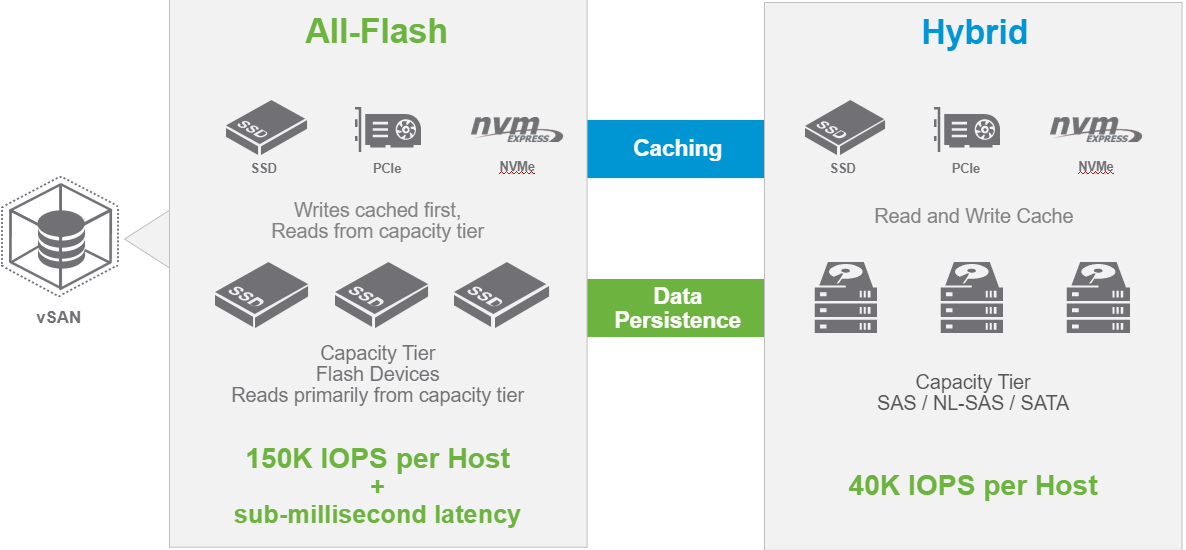
\includegraphics[width=0.6\textwidth]{imaxes/cap2recursos/rendimientoVSAN.png}
        \caption{Configuración \textit{All-Flash} y configuración \textit{Hybrid} en vSAN}
        \label{fig:performance-Hybrid-AllFlash-vSAN}
    \end{figure}
    \FloatBarrier
\end{subsubsection}

\begin{subsubsection}{VMware NSX-T}
    VMware NSX-T virtualiza la red del SDDC. Abstrae los componentes físicos de la red para generar una red virtual desacoplada de la infraestructura física que se puede configurar sin modificar la red física, para ello aporta servicios de red virtualizados y la posibilidad de crear y extender subredes. Internamente está formado por varias instancias de \textbf{NSX-T Manager Appliance} que a su vez se compone de \textit{NSX-T Manager} y \textbf{NSX-T Controller}. El primero es el punto de acceso a la configuración de VMware NSX-T y el que almacena y transmite la configuración establecida, el segundo controla las redes y servicios virtuales aportando la información y configuración necesarias para que gestionen el tráfico correctamente y obteniendo estadísticas sobre este. El control del tráfico y la monitorización de las conexiones se hace desde el componente \textbf{Transport Node} (TN) con la información que recibe de las instancias de NSX-T Controller. Existen dos tipos de TNs, \textbf{Hypervisor Transport Node} que son nodos con ESXi instalado y que están configurados para correr los servicios de VMware NSX-T, y \textbf{NSX-T Edge Node} que se trata de una \textit{appliance} instalada en una VM o sobre un nodo físico para proveer un conjunto de servicios de red centralizados para las redes virtuales de VMware NSX-T.
\end{subsubsection}
\begin{subsubsection}{VMware vRealize Suite}
    VMware vRealize Suite agrupa un conjunto de productos que si bien no son obligatorios para desplegar VCF, aportan funcionalidades extra que completan la formación del SDDC. Los productos que se utilizarán en este proyecto son \textbf{vRealize Suite Lifecycle Manager} dedicado a gestionar el desliegue, actualizaciones, certificados y licencias de los productos que forman VMware vRealize, \textbf{Workspace One Access} dedicado a gestionar los usuarios y ser el punto de acceso centralizado de las aplicaciones de VMware vRealize y, finalmente, \textbf{vRealize Automation} el cual permite a los usuarios del SDDC diseñar y aprovisionar un conjunto de recursos de la infraestructura según sus necesidades y de forma automatizada mientras el administrador puede limitar la cantidad de recursos que se consumen.
\end{subsubsection}
% \begin{itemize}
    % \item \textbf{SDDC Manager}: gestiona el ciclo de vida de todos los componentes del sistema, incluyendo el proceso inicial de despliegue de Cloud Foundation, su configuración y aprovisionamiento, y las actualizaciones. Monitoriza los recursos físicos y lógicos de la infraestructura, facilita su configuración y permite añadir nuevos recursos cuando sea necesario. \iffalse Todo esto lo realiza mediante flujos de trabajo que facilitan la detección de orígenes de errores.\fi
    % \item \textbf{vSphere}: ya está incluído en el servicio actual [\ref{subsec:softwareinstalado}].
    % \item \textbf{VMware vSAN}: componente clave que virtualiza el almacenamiento. Como ya se ha explicado, el almacenamiento del servicio actual está configurado con LUNs que se deben gestionar individualmente en una capa distinta a los componentes software, provocando que su configuración sea más compleja y costosa. El objetivo de VMware vSAN es gestionar de forma automatizada y desde un único lugar el sistema de almacenamiento de la infraestructura, tratando toda la capacidad y recursos de almacenamiento como un único elemento, eliminando así la necesidad de tener que crear LUNs aisladas, consiguiendo abstraer la configuración de almacenamiento de la capa física en la capa de software y permitiendo establecer políticas de almacenamiento desde cada máquina virtual para adecuarlo a las necesidades de cada una, sin tener que editar la configuración real del entorno físico. Así el rendimiento de los recursos de almacenamiento es más eficiente, flexible y su configuración se integra dentro del mismo servicio junto con la gestión del resto de componentes. \\
    % En VMware vSAN, en lugar de tratar el almacenamiento de forma independiente este pasa a estar ligado a cada host, es decir, cada uno de los nodos tiene asignados hasta cinco grupos de discos. Estos grupos de discos pueden ser de tipo \textit{Hybrid}, donde se combinan discos duros SSD y HDD, o \textit{All-Flash}, donde todos los discos son de tipo SSD. Dentro de cada grupo, los discos se dividen en dos tipos con distintas funciones, el disco de caché y el disco de capacidad\cite{operacionesVSAN}:
    %     \begin{itemize}
    %         \item \textbf{Caché}: Hay uno en cada grupo. Realiza la función de memoria caché y se encarga de escribir los datos persistentes en los discos de capacidad.
    %         \item \textbf{Capacidad}: Puede haber hasta siete discos en cada grupo. Almacena los datos persistentes del entorno.
    %     \end{itemize}
    % En cada grupo de discos la gestión de la \underline{lectura y escritura} de datos se hace de la siguiente forma:
    %     \begin{itemize}
    %         \item \textbf{Lectura}: En el caso de la solución \textit{Hybrid}, si el dato que se busca no está en el disco de caché entonces se busca en los discos de capacidad y después se incorpora al disco de caché. Con la solución \textit{All-flash}, los datos se leen siempre directamente de los discos de capacidad sin que estos sean escritos en el disco de caché dejando a este completamente libre para las operaciones de escritura. Gracias a esto, la estructura \textit{All-flash} ofrece mayor rendimiento respecto a la \textit{Hybrid}.
    %         \item \textbf{Escritura}: Tanto en la solución \textit{Hybrid} con en la \textit{All-flash}, el host ESXi primero escribe en el disco de caché, este le responde con una confirmación de escritura y más tarde vSAN se encarga de escribir ese dato en los discos de capacidad cuando el disco de caché está casi completo o cuando el dato lleva un tiempo sin ser utilizado.
    %     \end{itemize}
    %     \begin{figure}[h!]
    %         \centering
    %         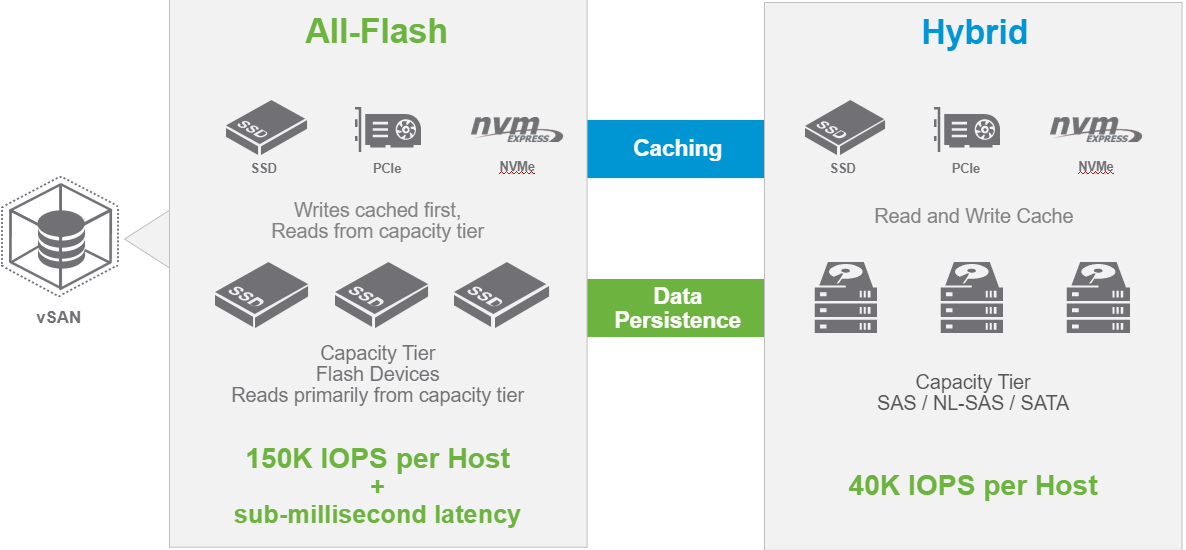
\includegraphics[width=1\textwidth]{imaxes/cap2recursos/rendimientoVSAN.png}
    %         \caption{Almacenamiento All-Flash vs. Híbrido en vSAN}
    %         \label{fig:rendimientoVSAN}
    %     \end{figure}
    %     \FloatBarrier
    % Los hosts acceden al \textit{datastore} de vSAN mediante protocolo IP en una red accesible por todos los nodos. \\ 
    % Este componente permite reducir las tareas de gestión del almacenamiento físico ya que ya no es necesario hacer ajustes en la capa física para cumplir unos requisitos en la capa software.
   
%     \item \textbf{VMware NSX-T}: otro de los componentes clave. Tiene un papel similar a vSAN, pero en este caso se encarga de virtualización de los componentes físicos de la red de la infraestructura, es decir, abstrae los componentes de la red para desacoplar la configuración de la red física y la red virtual del SDDC simplificando así las operaciones en la infraestructura física. Con esto, los administradores pueden configurar la red del SDDC sin tener en cuenta el equipamiento físico ya que trabajan con una red virtual independiente de la red física sobre la que funciona.
%     % \iffalse
%     % Incluye servicios de red como firewall, elimina el tráfico  DNS, DHCP, VPN, NAT, enrutamiento, balanceo de carga, o switching, que permiten reducir la cantidad de dispositivos físicos de red.\\
%     % \fi
%     Los componentes de VMware NSX-T se agrupan en tres capas/planos\cite{componentesNSX}:
%     \begin{itemize}
%         \item \textbf{Management Plane}: desde este punto se gestiona la conectividad, seguridad y operaciones de los componentes del sistema a través de un inventario de objetos, proporciona una interfaz y una API para acceder acceder a los componentes de VMware NSX-T, almacena y transmite la configuración del sistema al \textit{Control Plane} y obtiene información del sistema como estadísticas de uso. Estas funciones son implementadas por el componente \textbf{NSX-T Manager}.
            
%             % \begin{itemize}
%             %     \item \textbf{NSX-T Manager}: es el punto desde donde se administran todos los componentes de NSX. Existe una instancia de NSX Manager por cada instancia de vCenter Server. Contiene los archivos necesarios para desplegar el resto de componentes de NSX (NSX Edge Services Gateway y NSX Controller), y, cuando es creado, se encarga de habilitar las funcionalidades VXLAN sobre capa 2, Distributed Router y \textit{User World Agent} (UWA) en todos los hosts ESXi. Genera certificados para cada instancia de NSX Controller y host ESXi que utiliza para asegurar las comunicaciones en el \textit{Control Plane}.
%             % \end{itemize}
%         \item \textbf{Control Plane}: este plano comunica al cada componente la configuración establecida desde \textit{Management Plane}. Además, se encarga de obtener información sobre la topología de la red desde el \textit{Data Plane}. Este plano se divide en dos partes:
%             \begin{itemize}
%                 \item \textit{Central Control Plane} (CCP): implementado por un cluster de varias VM donde cada una contiene el componente \textbf{NSX-T Controller}, el cual es el encargado de controlar las redes virtuales existentes y de proveer de configuración a otros componentes como \textit{logical switches}, \textit{logical routers} y \textit{edge nodes}. El componente \textbf{NSX-T Controller} está integrado, junto con el componente \textbf{NSX-T Manager}, en una única \textit{appliance} denominada \textbf{NSX-T Manager Appliance}
%                 \item \textit{Local Control Plane} (LCP): este plano lo implementan los \textbf{transport nodes} y es responsable de monitorizar los enlaces locales y de reenviar entradas de configuración a los componentes del \textit{Data Plane}.
%             \end{itemize}
%             % \begin{itemize}
%             %     \item \textbf{NSX Controller}: se encarga de almacenar y transmitir información sobre la red a cada hosts ESXi. Provee la información sobre los segmentos VXLAN existentes, la información sobre el enrutamiento en la red virtual, almacena las tablas ARP, MAC y VTEP. Esto permite que se pueda eliminar el tráfico Broadcast de las redes VXLAN, ya que este tipo de tráfico es generado por las máquinas virtuales y capturado por el host ESXi que lo reenvía a la instancia de NSX Controller para obtener la información requerida. También elimina la necesidad de configurar los protocolos Multicast Routing y \textit{Protocol Independent Multicast} (PIM) para implementar redes VXLAN. Se despliegan tres instancias de NSX Controller para proveer alta disponibilidad.
%             %     \iffalse
%             %     \item \textit{User World Agent} (UWA): proceso que usa una instancia de NSX Controller para comunicarse con cada host ESXi a través de su dirección IP en la red
%             %     \fi
%             %     \item \textbf{Logical Router Control}: se trata de una máquina virtual que se genera cada vez que se crea el componente Distributed Logical Router. Busca routers adyacentes, tanto físcos como virtuales, para formar tablas de enrutamiento que se envían a NSX Manager que las comunica al resto de dispostivos.
%             % \end{itemize}
%         \item \textbf{Data Plane}: este plano es responsable de retransmitir el tráfico por la red basándose en lass tablas  y reglas generadas por el \textit{Control Plane}. También informa al \textit{Control Plane} sobre la topología de la red, recopila estadísticas a nivel de paquete y controla el estado de los enlaces para resolver posibles fallos. En definitiva, el \textit{Data Plane} se centra en como gestionar los paquetes que circulan por la red. Está implementado por dos tipos de \textbf{transport nodes} (TN):
%         \begin{itemize}
%             \item \textit{Hypervisor Transpor Node}: son los hosts con el hipervisor ESXi y que utilizan VMware NSX-T para proveer servicios de red a las VM que funcionan sobre sobre el host.
%             \item \textit{VMware NSX-T Edge Node}: también llamado \textit{Edge Node}, se trata de una \textit{appliance} instalado sobre un servidor físico o en forma de VM, que provee al entorno de una serie de servicios de red centralizados.
%         \end{itemize}
% VMware NSX-T inlcuye otros componentes:
%     \begin{itemize}
%         \item \textbf{NSX-T Virtual Distributed Switch} (N-VDS): funciona sobre el hipervisor ESXi de cada host y es el encargado de retransmitir el tráfico entre las VM que se encuentran dentro de un mismo \textit{transport node} y desde una VM a la red física de la infraestructura.
%         \item \textbf{Logical Router}: Integra dos componentes, \textbf{Distributed Router} (DR) proporciona conectividad entre las redes virtuales que se crean dentro del SDDC funciona de forma distribuída en los \textit{transport nodes}), y \textbf{Service Router} (SR) da conectividad hacia redes redes externas al SSDC y ofrece una serie de servicios centralizados, NAT y DHCP entre otros.
%         \item \textbf{Logical Firewall}: NSX-T permite establecer reglas para gestionar el tráfico de entrada y de salida del SDDC. Estas reglas se pueden establecer a nivel de \textit{Layer 2} o \textit{Layer 3} de la red.
%         \item \textbf{Logical Load Balancer}: se encarga de distribuir el tráfico que recibe a los componentes correspondientes, permitiendo desacoplar el acceso a un servicio de su implementación. Esto permite que un servicio se pueda escalar y ofrecer alta disponibilidad.
%     \end{itemize}
        
% \FloatBarrier
        % \item \textbf{Data Plane}: está controlado por NSX Virtual Switch el cual extiende las funcionalidades de vSphere Distributed Router, clave para la virtualización de la red. Estas características son:
        %     \begin{itemize}
        %         \item \textbf{Distributed Firewall}: filtra el tráfico con un servicio de Firewall, permitiendo segmentar las máquinas virtuales estableciendo políticas según sus características. Está distribuído en todos los hosts ESXi.
        %         \item \textbf{VXLAN}: protocolo que habilita la creación de redes virtuales sobre una red IP ya existente. Es gestionado a través de \textit{VXLAN Tunnel EndPoints} (VTEP) repartidos por cada host ESXi para encapsular el tráfico saliente de las máquinas virtuales con la cabecera de la red VXLAN.
        %         \item \textbf{Distributed Logical Router} (DLR): elemento que reside en el hipervisor de cada host ESXi y que se encarga de enrutar el tráfico entre las máquinas virtuales a través de la red virtual del SDDC sobre VXLAN. Soporta los protocolos de enrutamiento dinámico BGP y OSPF. DLR pasa a llamarse Universal Distributed Logical Router (UDLR) cuando se configura el mismo UDLR a través de varias \textit{regions} de un SDDC.
        %         \item \textbf{Logical Switch}: se definen dentro del componente vSphere Distributed Switch sobre un \textit{portgroup}. Crea segmentos de red ya que tiene una VXLAN asignada, es decir, un segmento/red VXLAN está delimitada por un Logical Switch. Está distribuido en cada host ESXi\footnote{El Logical Switch se extiende en toda la \textit{transport zone} de la VXLAN a la que pertenece, esta define el alcance de un segmento VXLAN que puede extenderse en varios clusters pertenecientes a una instancia de vCenter Server.}.
        %         \item \textbf{Edge Services Gateway} (ESG): es una máquina virtual que se encarga de enrutar el tráfico hacia redes externas al SDDC, por lo tanto está conectado con el DLR y con el dispositivo físico de enrutamiento de capa 3. Provee servicios perimetrales como SSL, NAT, DHCP, VPN y Load Balancing.
        %     \end{itemize}
    %\end{itemize}
    
        % \begin{figure}[h!]
        %     \centering
        %     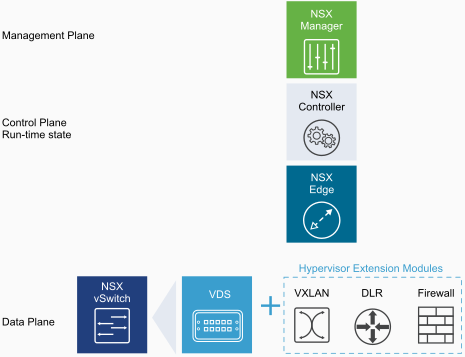
\includegraphics[width=0.55\textwidth]{imaxes/conceptosPrevios/planosNSX.png}
        %     \caption{Componentes de VMware NSX}
        %     \label{fig:planosNSX}
        % \end{figure}

        
    % \iffalse
    %     \item \textbf{NSX Manager}: es el punto de entrada de la comunicaión con la instancia de vSphere, se encarga de desplegar NSX Controllers y el resto de servicios de NSX, instala VXLAN en los hosts ESXi, \textit{distributed routers} y firewalls, se comunica con los NSX Controllers y genera certificados para que las comunicaciones con los hosts ESXi sean seguras.
    %     \item \textbf{NSX Controller}: establece el punto de control desde donde se distribuye la información sobre el enrutamiento lógico y de VXLAN hacia los hosts ESXi, existen varios nodos de este tipo para facilitar el escalado y alta disponibilidad de la infraestructura, comparte la información de red entre el resto de NSX Controllers, abstrae el uso de VXLAN sobre la red física y elimina el uso del protocolo ARP en redes VXLAN. 
    %     \item \textbf{NSX Virtual Switch}: gestiona los vSphere vSwitch Distibuted desplegados, proporcionando switching entre los hosts ESXi.
    %     \item \textbf{NSX Logical Router Control}: se despliega cuando se crea un Distributed Logical Router. Se encarga de buscar adyacencias para generar tablas de enrutamiento que envía a NSX Manager y a los NSX Cotrollers para que informen a cada Distributed Logical Router en cada nodo ESXi.
    %     \item \textbf{NSX Edge}: proporciona servicios múltiples servicios como firewall perimetral de capa 2 y 3, SSL, NAT, DHCP, VPN, balanceo de carga y alta disponibilidad.
    % \fi
    % \item \textbf{VMware vRealize Log Insight}: realiza la gestión de logs del servicio, dando visibilidad a todas las operaciones del servicio, generando análisis del sistema. Esto permite tener mayor conocimiento de los riesgos, eficiencia y uso de recursos, a parte de facilitar la búsqueda de orígenes de errores. Está formado por los siguientes componentes:
    % \begin{itemize}
    %     \item \textbf{Nodo Master}: es el único nodo que se despliega en el modo \textit{standalone}, en ese caso se encarga de la obtención de logs de los servicios de VMware Cloud Foundation y de entregar la información almacenada al cliente. Cuando se despliegan más nodos, se encarga de gestionar la creación, elimación y actualización de los nodos worker.
        
    %     \item \textbf{Nodo Worker}: es un nodo opcional que se crea para proporcionar alta disponibilidad y escalar el entorno. En este tipo de nodo se delegan la entrega de la información almacena al cliente y la obtención de logs de cada host ESXi.
        
    %     \item \textbf{Load Balancer}: simplifica la configuración de la alta disponibilidad cuando hay nodos worker desplegados. Se encarga de recibir las peticiones de los clientes, de entregarlas a los nodos worker y de enviar la respueste. También gestiona el balanceo del tráfico entrante entre todos los nodos y de escoger el nodo \textit{master}. Se ejecuta en uno de los nodos de VMware vRealize Log Insight.
    % \end{itemize}
    
%     \item \textbf{VMware vRealize Automation}: se trata de un componente opcional que permite automatizar el despliegue de máquinas virtuales, procesos y aplicaciones reduciendo la complejidad y eliminando tareas manuales. Esto acelera la entrega del servicio gracias a que las tareas de aprovisionamiento y entrega de recursos y aplicaciones son más rápidas permitiendo establecer políticas de seguridad y control. Internamente, este servicio \underline{cuenta con los siguientes componentes \cite{vRealizeAutomation}} para cumplir con sus funciones:
%     \begin{itemize}
%         \item \textbf{vRealize Automation Appliance}: contiene un portal donde los usuarios pueden acceder y gestionar y aprovisionar servicios cloud bajo demanda, un servicio de autenticación y una interfaz para gestionar este componente. 
%         \item \textbf{IaaS Web Server}: realiza las tareas de administración de la infraestructura que se requieren desde el portal de vRealize Automation Appliance.
%         \item \textbf{Microsoft SQL Server}: se utiliza para almacenar información sobre los elementos de IaaS y sobre las máquinas virtuales controladas por vRealize Automation Appliance.
%     \end{itemize}
% \end{itemize}













% \iffalse
% \subsubsection{OpenStack}
% Es una plataforma constituída por tres proyectos, uno dedicado a la gestión de la red, otro a la gestión del cómputo, y otro a la gestión del almacenamiento. Para poder desplegarlo sobre los componentes de VmWare instalados en nuestra infraestructura son necesarios tres plugins específicos para el software de VmWare. OpenStack aporta una API a través de la cual es posible gestionar los recursos virtuales y el aproivisionamiento.

% \subsubsection{Apache CloudStack}
% \fi
\end{subsection}
\end{section}
